% !TEX program = xelatex

\documentclass[12pt,a4paper]{article}

\usepackage{amsthm,amsfonts,amssymb,bm}
\usepackage[fleqn]{amsmath}

% Page settings
\addtolength{\textheight}{2.0cm}
\addtolength{\voffset}{-2cm}
\addtolength{\hoffset}{-1.5cm}
\addtolength{\textwidth}{4.0cm}

%\allowdisplaybreaks

%\usepackage{subeqnarray}
\usepackage{mathrsfs}
%\usepackage{color}
%\usepackage{url}
%\usepackage{ulem}
\usepackage{indentfirst}   % Indent first line of a paragraph
%\usepackage{textcomp}




%%Here is the configuration for chinese. setmainfont is the default font of the text.
\usepackage[cm-default]{fontspec}
\usepackage{xunicode}
%\usepackage{xltxtra}
%\setmainfont{"微软雅黑"}
%\setsansfont[BoldFont=SimHei]{KaiTi_GB2312}
%\setmonofont{NSimSun}



\XeTeXlinebreaklocale "zh"
%\XeTeXlinebreakskip = 0pt plus 1pt

% Figure, Diagram, Caption settings
%\usepackage{tikz}
%\usetikzlibrary{mindmap,trees}
\usepackage{graphicx}
%\usepackage{graphics}
%\usepackage[hang,small,bf]{caption}
%\setlength{\captionmargin}{50pt}

% Redefine some fonts.
%\newfontfamily\heiti{"黑体"}
%\newfontfamily\fs{"仿宋"}
%\newfontfamily\yahei{"微软雅黑"}


\graphicspath{{Figure/}}

\begin{document}
\title{A Note on Density of Dust Sphere}
\author{MA Lei}
\maketitle

% Redefine some math commands and environments.

\newcommand{\dd}{\mathrm d}
%\newcommand{\HH}{\mathcal H}
%\newcommand{\CN}{{\it Cosmologia Notebook}}
\newenvironment{eqnset}
{\begin{equation}\left \bracevert \begin{array}{l}}
{\end{array} \right. \end{equation}}

\newenvironment{eqn}
{\begin{equation}\left \bracevert \begin{array}{l}}
{\end{array} \right. \end{equation}}




This simple article is aimed to calculate the density of a dust sphere and show some interesting features.

Imagine a dust sphere in space. It has a Schwarzschild since it's spherical symmetric,

\begin{equation}
\mathrm ds^2 = -(1-\frac{2m(r)}{r})c^2 \mathrm dt^2 + (1- \frac{2m}{r})^{-1}\mathrm d r^2 +r^2 (\mathrm d\theta^2 + \sin^2\theta \mathrm d\phi^2)
\end{equation}

To get the density, we have to calculate the volume. Use a time orthonormal space and integrate over a shpere.

\begin{eqnarray}
V(R,M)&=&\int \frac{1}{\sqrt{1-\frac{2m(r,M,R)}{r}}} r^2 \sin\theta \mathrm dr\mathrm d\theta\mathrm d\phi \\
&=&4\pi^2 \int \frac{1}{\sqrt{1-\frac{2m(r)}{r}}}r^2 \mathrm dr
\end{eqnarray}
where $m(r,M,R)$ is the mass distribution,  $M$ is the total mass of the sphere, $R$ is the total radius (in unit of the coordinate of Shwarzschild metric) of the sphere.

Choose a specific mass uniform distribution, 
\begin{equation}
m(r,M,R)=\frac{4/3 \pi r^3}{4/3 \pi R^3}=(\frac{r}{R})^3 M
\end{equation}

Then the volume can be simplified,
\begin{equation}
V=4\pi^2 \int \frac{1}{\sqrt{1-2 M \frac{r^2}{R^3}}}r^2\mathrm dr
\end{equation}

Finally, the density of the dust can be calculated using the defination$\rho=M/V$。

It would help us to understand the behavior of this density if we plot the $\rho \sim R$ and $\rho \sim M$ figure.


Figure (\ref{fig:FixR}) shows the density of the dust with $R=1$ while change total mass $M$.
\begin{figure}[!htbp]
\centering
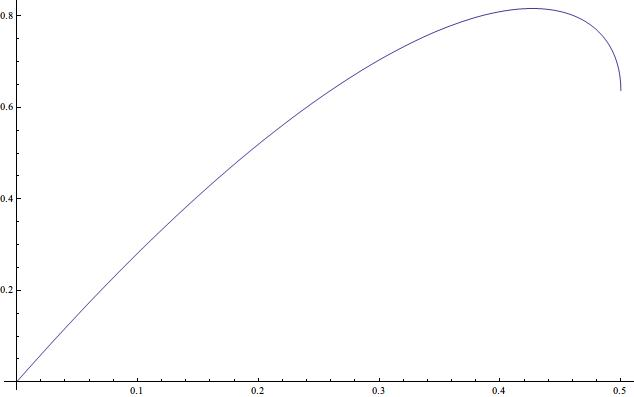
\includegraphics[width=400pt]{DustBlackHole_FixR.jpg}
\caption{A dust sphere with radius 1 and varying mass.}\label{fig:FixR}
\end{figure}

Now it is clear that for a raduis 1 sphere, the density it increases at first and then reaches it's peak value 0.816 at point $M=0.427$ if we add mass to it and keeps it's mass distribution not changed. Then the density drop to $2/\pi$ when $M=0.5$. It forms a black hole if we add more mass. It is really clear from this figure that the slope could be infinite at $M=0.5$ and a calculation confirms this guess.

This is weird. If the density really goes to zero, where does the mass go? How does the volume change when the dust forms a black hole? From the expression of density, the volume becomes infinity. However, this is a result of gravity. Can we reform the expression so that the effect is on mass?

The explicit density is
\begin{eqnarray}
\rho(M,R)&=&\frac{-2 R\sqrt{M(-2M R^2+R^3)}+\sqrt 2 R^3 \arcsin (\sqrt{2 \frac{M}{R}})}{8 (\frac{M}{R})^{3/2}}\label{eqn:densityMR}
\end{eqnarray}

In equation (\ref{eqn:densityMR}), the mass should be gravitational mass because it changes the background metric through gravity. If the gravitational mass does change, then the gravitational mass should be zero too. This is not easy to model this gravity since we have to keep the expression of both mass, volume and density consistent. I have no idea on this now.

One more thing, the gravity theory should fit the observable universe.

Figure (\ref{fig:FixM}) is the change of density when the radius is changed for a $M=1$ dust sphere.
\begin{figure}[!htbp]
\centering
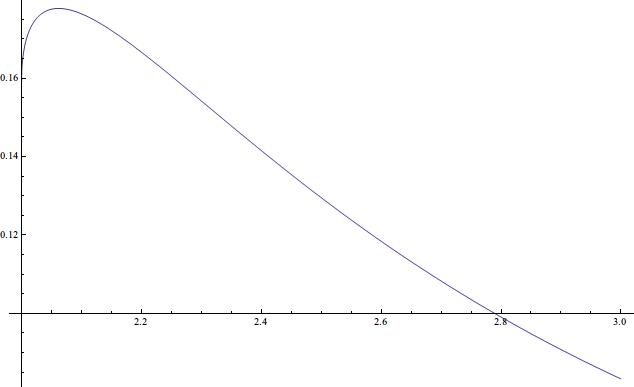
\includegraphics[width=400pt]{DustBlackHole_FixM.jpg}
\caption{Dust with mass $M=1$.}\label{fig:FixM}
\end{figure}

The peak point of figure (\ref{fig:FixM}) is ($R=2.062$, $\rho=0.178$). At the critical point occurs at $R=2$, where the density is $\rho=2/\pi$. This is consistent with figure (\ref{fig:FixR}).



The full behaviour of the density is shown in figure (\ref{fig:3D}).
\begin{figure}[!htbp]
\centering
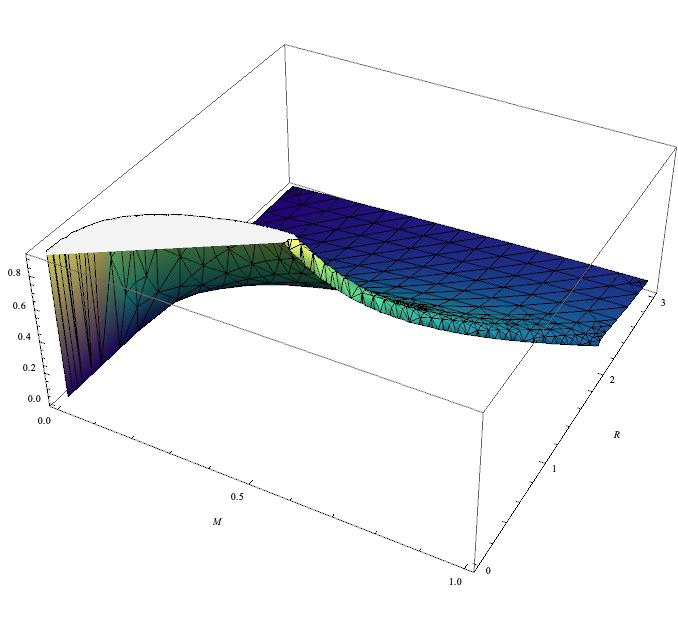
\includegraphics[width=400pt]{DustBlackHole_3D.jpg}
\caption{Full behaviour of the density.}\label{fig:3D}
\end{figure}


\end{document}